\chapter{Introduction}
\label{ch:introduction}
Throughout human history we have been driven to understand the world around us. It is surely one of the characteristics that defines us as a species. Coupling that curiosity with our ability to create and construct incredible machines has allowed us to probe some of the most elusive parts of our Universe. From the Hubble Telescope taking in images of the earliest moment of our Universe to the Large Hadron Collider probing the most fundamental particles that we currently know, we have been wildly successful at fulfilling that drive to understand.

Despite that success, there are many issues that continue to elude us. Dark matter and dark energy, which is believed to make up 96\% of our Universe, are phenomena we know almost nothing about. Another puzzle that we currently have no tangible explanation for is the asymmetry of matter to anti-matter. In the very early Universe there were equal amounts of matter and anti-matter, yet today our visible Universe seems to be comprised primarily of matter and not anti-matter. Even of the matter that we know, we know surprisingly little about its structure and composition.

Atoms make up much of our visible Universe. Since the early 1900's we have known these atoms to be made of protons, neutrons and electrons. The discovery of protons and electrons essentially occurred in the late 19th Century, but the neutron was not discovered until 1932 by Sir James Chadwick. The neutron was not just found later than the electron and proton, but we also know much less about it. The electron is well-known in the physics community to be a near point-like particle with no constituents, but the proton and neutron have been proven to be made of constituent particles.

\section{Quantum Physics and the Standard Model in a Nutshell}
Knowing exactly what makes up these protons and neutrons relies on knowledge of the Standard Model of Particle Physics, or sometimes referred to as just the Standard Model. This model, developed in stages throughout the latter half of the 20th Century, essentially lays out the existence of all possible fundamental \footnote{The word "fundamental" here means that they are not made of constituent particles.} particles in the Universe.

There are 17 particles in the Standard Model (outlined in Fig. \ref{fig:standard_model}). These 17 can first be broken down into two subgroups called bosons and fermions. Bosons follow what is known as Bose-Einstein statistics, which essentially states that they can occupy the same space at the same time. In the language of quantum physics, two bosons can be described by the same quantum numbers. The bosons are all force carriers. Photons are the force carriers for the electromagnetic force. Gluons carry the strong force. W and Z bosons are the force carriers for the weak force. Higgs boson is a bit different in that it is not necessarily a force carrier. Its existence is tied to the breaking of electroweak symmetry \footnote{In the early Universe, the electromagnetic and weak forces were one force. As the Universe began to cool, the symmetry that kept these two forces together broke. The Higgs boson essentially facilitated that breaking.} and it gives fermions their mass.

\begin{figure}[h!]
	\centering
	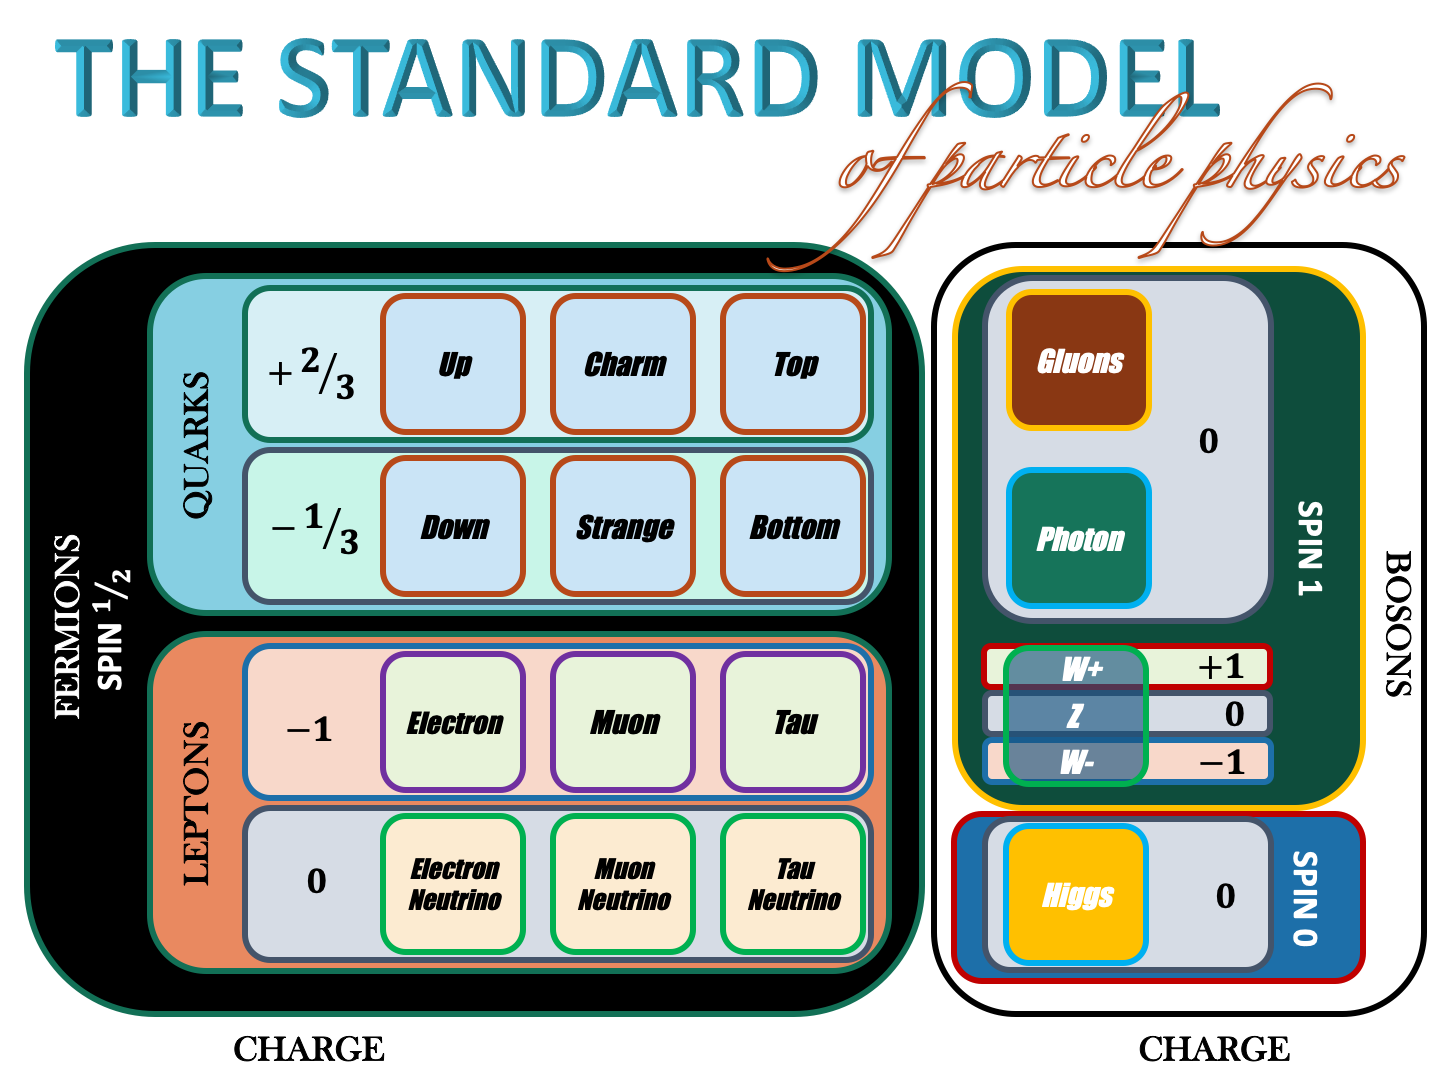
\includegraphics[width=0.8\linewidth]{figures/standard_model.png}
	\caption{The 17 fundamental particles of The Standard Model of Particle Physics.}
	\label{fig:standard_model}
\end{figure}

The other subgroup is fermions, which are 12 particles that obey a Fermi-Dirac statistical rule called the Pauli Exclusion Principle. Developed by Enrico Fermi, Paul Dirac and Wolfgang Pauli, this rule states that fermions cannot occupy the same place at the same time. Again in quantum physics language, no two fermions can be described by the same quantum numbers. There are two types of fermions in the Standard Model: 6 quarks and 6 leptons. Leptons, which include electrons, pions, tau and their associated neutrinos, cannot combine to make larger structures. Quarks, on the other hand, do combine to make larger structures, like protons, neutrons, atoms, molecules, people and light posts. They also obey the exclusion principle, which is why walking into a light post hurts. You both cannot be in the same place at the same time.

Quantum numbers, the things that help define the difference between fermions and boson, are conserved quantities that describe a quantum system. More precisely, quantum numbers are the eignenvlaues of operators that commute with the Hamiltonian. These quantum numbers can describe things like angular momentum, spin and parity. The namesake to these numbers and this entire field of physics comes from the fact that many of these quantities often exist in steps of discrete quantities ($e.g.$ integer or half-integer steps), thus quantized.

One of those quantized observables is something called spin. Because these fundamental particles are so incredibly small, they are considered featureless (or point-like). Therefore many of these quantum numbers have no physical meaning, they are simply mathematical constructs that tend to correspond to something physical we are familiar with. The spin quantum number is no exception. Fundamental fermions, as seen in Fig. \ref{fig:standard_model}, have spin $1/2$, while fundamental bosons have integer spin of 0 or 1. Two, three or more quarks combine by way of the strong force. Two quarks combine to make something called mesons ($e.g.$ pions and kaons) and their spin states combine to form an overall integer 1, which also makes them bosons. Three quarks combine to make baryons ($e.g.$ protons and neutrons), which have spin $1/2$ or $3/2$ making them fermions as well.

Charge is another important quantized observable. When three quarks combine to make a proton or neutron, their charges also combine. A proton, for example, is made of two up quarks\footnote{Quark names are essentially meaningless. There is no physical characteristics that warrant a quark being called up or strange. They were simply given a name that stuck.} (each with charge $+2/3$) and a down quark (charge $-1/3$), so its overall charge is $+1$. A neutron is made of two down quarks and an up quark, so its charge is zero.

\section{The Trouble with Understanding the Nucleon}
Protons and neutrons make up the nucleus of an atom so they are called nucleons. These nucleons are not just made of three stationary quarks, but are very dynamic and busy particles. These three quarks that define whether it is a proton or neutron called valence quarks. However, there are also quark-antiquark pairs that are in a constant state of creation and annihilation, called sea quarks. Then there are gluons which are carriers of the strong force connecting quarks together. All of these particles have momenta and collectively define the structure of the nucleon. The trouble in physics has been defining this structure and the size of these nucleons as well as the momentum distribution of the fundamental particles that exist within it.

There has been a lot of effort exploring the structure and momentum distribution of the proton, yet there are some major puzzles that still exist. One of the most famous has to do with the proton spin called the "proton spin crisis". This crisis refers to our collective inability to explain how all of the particles that exist in the proton conspire together to always give the proton spin $1/2$. Less famous puzzles include knowing the proton radius, where its mass comes from, and what the momentum distribution is of its fundamental constituent particles.

All of these puzzles also exist for the neutron, except with even less understanding. Whereas protons are easily confined to form targets for experiments, neutrons are not. Neutrons alone decay in about 15 minutes, and because they do not have electric charge, cannot be easily confined. One of experiments that set out to confirm or reject theories attempting to explain one of puzzles, the structure of the neutron and the momentum distribution of its constituents, is called the Barely Off-shell Nucleon Structure Experiment at 12 Giga-electron Volts (or BONuS12).
 
 \section{Scattering Experiments and BONuS12}
 There was an original BONuS Experiment that ran in 2005 that operated around the same concept of BONuS12, just with less energy at 6 Giga-electron Volts (or GeV). In order to probe the enigmas of particles that are on the order of 50 trillion times smaller than a grain of sand, particle and nuclear physicists often use scattering experiments. These experiments accelerate particles to known energies and collide them on to a target.
 
 The collision of accelerated particle and target causes them both to scatter and, in some cases, fragment. The scattered particles resulting from the collision then enter particle detectors where information like energy, position, momentum, and time are gathered by exploiting various physics processes. With this information physicists can extract things like the structure of nucleon or the momentum distribution of the fundamental constituents within it.
 
 The Thomas Jefferson National Lab (JLab) in Newport News, Virginia contains a electron accelerator used for scattering experiments meant to explore nuclear and subatomic matter. Here is where, in 2005, the first BONuS Experiment ran in JLab's Experimental Hall B. The goal of that experiment was to explore the structure of the neutron and know more about the momentum distribution of the quarks and gluons inside. The results of the experiment made progress in narrowing error bars, which helped to begin confirming or denying some theories that exist attempting to attach values to these characteristics.
 
 Jefferson Lab, in 2012, began an energy upgrade to bring the electron beam energy to 12 GeV, and with that came the development of an upgraded BONuS Experiment (called BONuS12). Just like the BONuS6 Experiment (that is the original BONuS Experiment which ran at 6 GeV), it is designed to explore the structure of the neutron and the momentum distribution of its fundamental constituent particles. The changes were made to improve the coverage of the detector, the momentum range that the RTPC can detect, and will extend the fraction of quark momentum to neutron momentum closer to one.
 
\section{Inclusive Deep Inelastic Scattering Data Analysis on Run Group A Data}
Throughout the rest of this work we will primarily discuss BONuS12, the physics necessary to understand its operation, and the efforts made to make the BONuS12 Experiment operational before it runs in Spring 2020. As a part of that comes the need to confirm that data coming in from Hall B experiments at JLab makes sense and is calibrated correctly. 

While the BONuS12 RTPC will detect scattered protons, the scattered electron will enter in to existing detectors in Hall B, so understanding that electron data is important. For that, a portion of this work will be dedicated to analyzing data from one of the first experiments that ran after the start of the 12 GeV physics era at JLab ($i.e.$ Run Group A). The process known as inclusive deep inelastic scattering will be examined since we know much about it. In particular, we will look at what is known as the cross section of the process and compare it to simulations that use well known values of that cross section. This will hopefully provide evidence that the detectors within Experimental Hall B, where the BONuS12 Experiment will run, are working correctly and are calibrated correctly.